\chapter{Rozmywanie regulatorów}

\section{Funkcje aktywacji}

Dla obu regulatorów dobrano identyczne funkcje aktywacjii dla trzech regulatorów lokalnych. Rozmywane one są względem wartości sterowana w poprzednim momencie. Zdecydowano się na to z dwóch powodów: po pierwsze układ może zmieniać swoje punkty pracy w zależności od warunków atmosferycznych otoczenia, rozmywanie po wyjściu naraża nas na wpływ takich odchyleń i spadek jakości regulacji; po drugie nieliniowość na obiekcie jest wprowadzana sterowaniem, tzn. obiekt (według tego co ustalono na projektach 1 oraz 2) jest w miarę liniowy, a jego właściwości nie mogły się zmienić, nieliniowość narzucana jest przez funkcję \verb|sendNonlinearControls|, która jakoby przerabia sterowanie tak, aby układ zachowywał się jak nieliniowy. \\

Pierwszy regulator lokalny będzie aktywny głównie w przedziale 0-50\% (na tym przedziale obiekt zachowuje się jak liniowy), drugi w przedziale 45-55\%, a trzeci głównie w przedziale 50-100\%, patrz rysunek \ref{fun_przyn}:

\begin{figure}[h!]
	\centering
	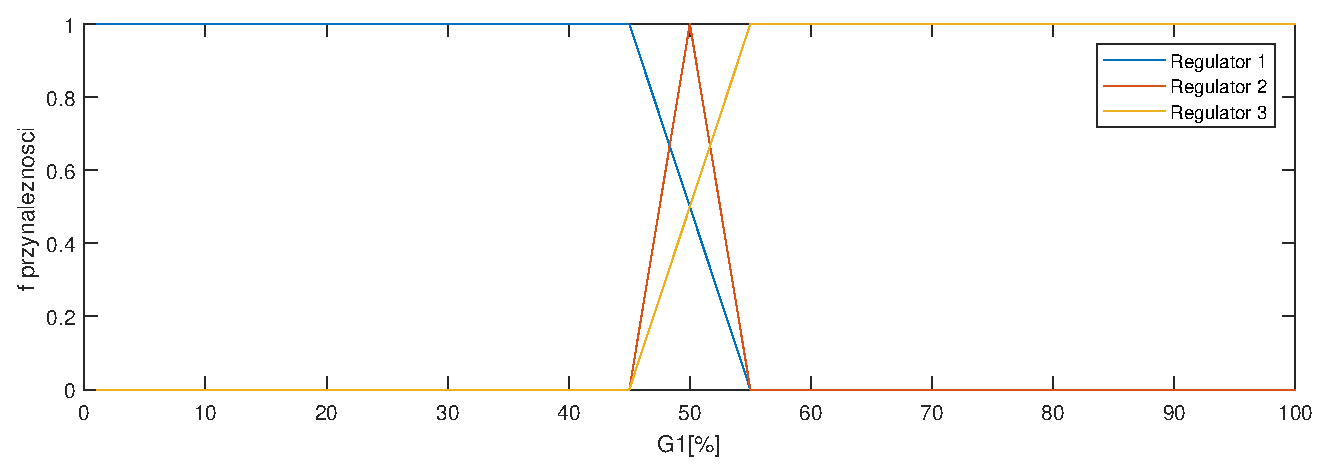
\includegraphics[scale=0.75]{Rys/Przynaleznosc.eps}
	\caption{Funkcje aktywacji regulatorów lokalnych}
	\label{fun_przyn}
\end{figure}

\FloatBarrier

\section {Rozmyty regulator PID}

\subsection{Algorytm}

W celu weryfikacji po